\mychapter{Teori}


\section{Kryptering}


\section{Blockchiffer}


\subsection{Körlägen}


\subsubsection{ECB}
\acrfull{ecb} är en av det enklaste körlägena som \acrshort{aes} använder.
\acrshort{ecb} i sig är ganska lätt att förstå och bygger i huvudsak bara på
att man tar varje block för sig och kör genom algoritmen, vilket väldigt
tydligt visas i Figur \ref{ecb-mode-enc} \& \ref{ecb-mode-dec}.
\footfullcite{modesofoperation}

\begin{figure}[H]
    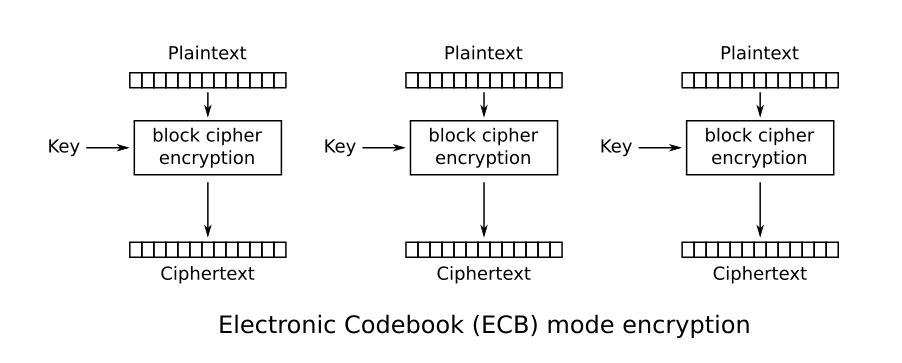
\includegraphics[width=\textwidth]{ECB_encryption.png}
    \captionsource{\acrlong{ecb} kryptering}{{\cite{ecb-mode-enc-ref}}}
    \label{fig:ecb-mode-enc}
\end{figure}

\begin{figure}[H]
    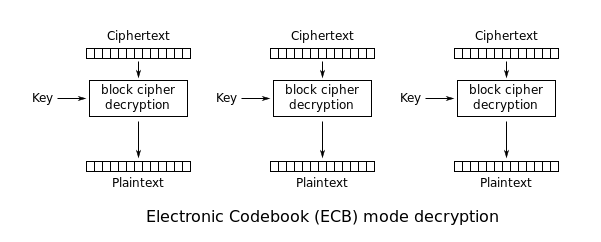
\includegraphics[width=\textwidth]{ECB_decryption.png}
    \captionsource{\acrlong{ecb} dekryptering}{{\cite{ecb-mode-dec-ref}}}
    \label{fig:ecb-mode-dec}
\end{figure}

\subsubsection{CBC}


\subsubsection{OFB}


\section{Symetrisk \& Asymmetrisk Kryptering}
Symetrisk och asymetrisk kryptering handlar om hur nycklar används i olika
krypteringsalgoritmer. För symetriska krypterings algoritmer så betyder detta
att samma nyckel är vad som används för både kryptering och dekryptering.

\footfullcite{symencrypt}

\section{AES}


\subsection{Finite Fields}


\subsection{AES S-Box}


\subsection{Struktur}


\subsubsection{SubBytes operation}
SubBytes operationen bygger på ...

\subsubsection{ShiftRows operation}


\subsubsection{MixColumns operation}


\subsubsection{AddRoundKey operation}


\subsection{Nyckel utökning}


\subsubsection{RotWord}


\subsubsection{SubWord}


\subsubsection{Rcon}


\subsection{AES-128bit}


\subsection{AES-192bit}


\subsection{AES-256bit}

